\section{Understanding Transient Server Failures}

Transient cloud servers, by their very nature have limited availability and are frequently preempted.
These preemptions are akin to fail-stop failures, and are often preceeded by a small advance warning (few seconds) to allow for graceful shutdowns.

Since preemptions can impact the availability, performance, and cost of running applications, in this section, we examine their preemption characteristics.
This modeling is important, because having a model of the availability can be useful in the context of predicting the running times of applications.
Cloud providers offer a large number of servers of different configurations and types.
Since transient server availability is fundamentally tied to supply and demand, the availability of servers of different types can be significantly different. 
Thus, selecting the ``right'' server type is crucial for minimizing the overall costs. 




\subsection{EC2 spot instances}

The earliest form of transient cloud instances.
In addition to having dynamic availability, also have dynamic pricing.
``Classic'' spot instances had price determining the availability, and thus a large amount of work was devoted to bidding and analyzing the prices.

However a recent change to the spot prices no longer allows these assumptions, rendering it impossible to obtain the \emph{exact} availability information from the prices alone.


\subsection{Google Preemptible VMs}

Launched in 2015.
Flat-rate discount of 80\% compared to on-demand servers.
Interesting availability SLA: the maximum lifetime is 24 hours, and can be preempted earlier as well.

In this paper we will look at these preemptible VMs and show how to model their availability.
Given the inability to use EC2 prices, we believe that our approach is more generalizable and robust.

\begin{figure}
  \centering
  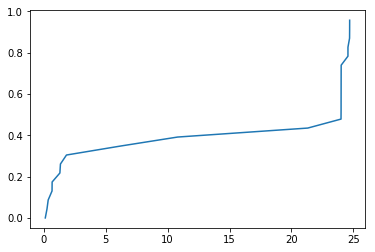
\includegraphics[width=0.4\textwidth]{../data/f20.png}
  \caption{CDF of lifetimes of Google Preemptible Instances }
  \label{fig:gcp1}
\end{figure}

There are some distinguishing characteristics of GCP preemptible VMs that makes their failure modeling challenging.
First is their flat pricing and no other signalling information about their preemption rates (MTBFs) that makes server selection difficult.




%%% Local Variables:
%%% mode: latex
%%% TeX-master: "paper"
%%% End:
